\section{Introduction}
Despite the widespread adoption of blockchains, a significant challenge remains unresolved: they are inherently slow. The latency from the moment a client submits a transaction to when it is confirmed in another client's view of the blockchain can be prohibitively long for certain applications. Notice that we define latency in terms of the blockchain \emph{liveness} property, referring to finalized, non-reversible outputs: once a transaction is received by a reader, it remains in the protocol's output permanently.
Moreover, we do not assume ``optimistic'' or ``happy path'' scenarios, where transactions might finalize faster under favorable conditions (such as having honest leaders or optimal network conditions).


Indeed, Nakamoto-style blockchain protocols require a large number of rounds in order to achieve consensus on a new block, even when considering the best known bounds~\cite{DBLP:conf/crypto/GaziRR23}. On the other hand, it is known that permissioned protocols for $n$ parties (out of which $t$ are corrupted) realizing traditional notions of broadcast and Byzantine agreement require at least $t+1$ rounds in the synchronous case~\cite{DBLP:journals/ipl/AguileraT99} and at least $2n/(n-t)$ rounds in the asynchronous case~\cite{DBLP:conf/focs/GarayKKO07}, even when allowing for digital signatures and probabilistic termination.


In a model where \emph{replicas} maintain the network, \emph{writers} submit transactions, and \emph{readers} read the network, the minimum latency is one network round trip, or $2\delta$, letting $\delta$ denote the actual network delay, as the information must travel from the writers to the replicas and then to the readers. More importantly, we want that any transaction from an honest writer appears in the output of honest readers within $2\delta$ time, regardless of the current value of $\delta$ and corrupted parties' actions.
In this context, we are motivated by the following question:

%\begin{center}
%	\emph{Can we perform payments -- and other tasks that blockchains are commonly used for -- in optimal latency?}
%\end{center}
\vspace{-2mm}
\begin{center}
	\emph{Can we realize tasks that blockchains are commonly used for with optimal latency?}
\end{center}
\vspace{-2mm}

We give a positive answer to this question with a protocol realizing \podtm, a new notion of consensus that trades off traditional agreement properties for optimal latency, while retaining sufficient security guarantees to realize important tasks (\textit{e.g.}, decentralized auctions).

\subsection{Our Contributions}
In order to motivate the notion of \podtm, we first introduce the architecture of our protocol, \podtm-core, which realizes this notion. To achieve the single-round-trip latency, our first key design decision is to eliminate inter-replica communication entirely. Instead, writers send their transactions directly to all replicas. Each replica maintains its own \emph{replica log}, processes incoming transactions independently, and transmits its log to readers on request. Readers then process these replica logs to extract transactions and relevant associated information. See Figure~\ref{fig:architecture} for a summary of the \podtm-core architecture.

\begin{figure}[ht]
    \centering
    \begin{minipage}{0.5\textwidth}
        \begin{center}
            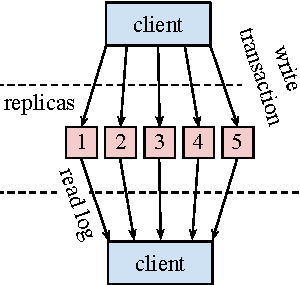
\includegraphics[width=0.55\textwidth]{figures/pod-architecture.pdf}
        \end{center}
    \end{minipage}%
    \hfill
    \begin{minipage}{0.5\textwidth}
        \caption{\podtm-core's simple architecture. A writing client (top) sends a transaction to all replicas (middle). Each replica appends it to its own log and transmits it to the reading client (bottom).}
        \label{fig:architecture}
    \end{minipage}
\end{figure}

This design raises two important questions. First, what meaningful information can readers derive from replica logs when replicas operate in isolation? Second, given that in two rounds even randomized authenticated broadcast is proven impossible~\cite{DBLP:conf/focs/GarayKKO07}, what capabilities can this -- necessarily weaker -- primitive offer? We demonstrate that, by incorporating simple mechanisms, such as assigning timestamps and sequence numbers to transactions, replicas can enable readers to extract valuable information beyond mere low-latency guarantees. Furthermore, we show how the properties of \podtm can enable various applications, including auctions (as shown in \Cref{sec:auctions}).
Specifically, a secure \podtm delivers the following guarantees (formally defined in \Cref{sec:pod-model}):
\begin{itemize}
    \item Transaction confirmation within $2\delta$, with each transaction assigned a \emph{\confirmed round}: we say that the transaction becomes \emph{confirmed} at the time indicated by the \emph{confirmed round}.
    \item Censorship resistance when facing up to $\beta$ Byzantine and $\gamma$ omission-faulty replicas, ensuring all confirmed transactions appear in every honest reader's output.
    \item A \emph{past-perfect round} can be computed by readers, such that the reader is guaranteed to have received all transactions that are or will be confirmed prior to this round, even though not all transactions are strictly ordered.
    \item Accountability for all safety violations, \textit{i.e.}, if any safety property is violated, at least $\beta + 1$ replicas can be identified as misbehaving.
\end{itemize}

In particular, our Protocol \podtm-core, presented in \Cref{sec:pod-core-const}, realizes the notion of \podtm with the properties above, supporting a continuum of two adversarial models: up to \beta Byzantine replicas and up to \gamma omission-faulty replicas, out of a total of $n > 5 \beta + 3 \gamma$ replicas.
Protocol \podtm-core requires no expensive cryptographic primitives or setup beyond digital signatures and a PKI registering replicas' public keys. We showcase \podtm-core's efficiency by means of experiments with a prototype implementation presented in \Cref{sec:evaluation}. Our experiments show that even with 1000 replicas distributed around the world, the latency achieved by our protocol is just under double (resp. about 5 times) the round-trip time between writer and reader clients with security against omission-faulty (resp. Byzantine) replicas.


\subsection{Technical Overview}
We consider that time proceeds in \emph{rounds}, and that parties (replicas and clients) know the current round, so we can express \emph{timestamps} in terms of rounds. The output of \podtm associates each transaction $\tx$ with timestamp values $\rmin \geq 0$ (minimum round), $\rmax \leq \infty$ (maximum round) and $\rconf$ (\emph{confirmed round}). We call these values the \emph{trace} of \tx, and they evolve over time.
Initially we have $\rconf=\perp$ but later we get $\rconf \neq \perp$, when a transaction is \emph{confirmed}. The protocol guarantees \emph{confirmation within $u$ rounds}, meaning that, at most $u$ rounds after $\tx$ was written, every party who reads the \podtm will see $\tx$ as confirmed with some $\rconf \neq \perp$.
The protocol also guarantees that $\rmin \leq \rconf \leq \rmax$, a property we call \emph{confirmation bounds}:
while each party reads different values $\rmin,\rmax,\rconf$ for the same $\tx$, \podtm guarantees that values read by different parties stay within these limits.

When clients \emph{read} the \podtm, they obtain a $\podtm$ data structure $\Pod = (\txSet, \rperf)$, where $\txSet$ is the set of transactions and their traces and $\rperf$ is a \emph{past-perfect} round. The \emph{past-perfection} safety property guarantees that
%if a transaction $\tx$ did not appear in $\txSet$, then no other party will ever read $\tx$ with confirmed round $\rconf'$ such that $\rconf' < \rperf$. This guarantees that,
\txSet contains \emph{all} transactions that every other honest party will ever read with a confirmed round smaller than $\rperf$.  A \podtm also guarantees \emph{past-perfection within $w$}, meaning that $\rperf$ is at most $w$ rounds in the past.

% For each transaction $\tx$ in \txSet, the reader obtains associated timestamps $\rmin,\allowbreak \rmax, \rconf$ and auxiliary data $\txcert$, which may evolve. The protocol guarantees \emph{confirmation within $u$ rounds}, meaning that, at most $u$ rounds after $\tx$ was written, every party who reads the \podtm will see $\tx$ as confirmed with some $\rconf \neq \perp$.
% Moreover, \podtm guarantees \emph{confirmation bounds}, ensuring that
% % if a party reads $\tx$ with minimum round $\rmin$ and maximum round $\rmax$, for every other party who reads $\tx$ with $\rconf' \neq \perp$, it holds that $\rmin \leq \rconf' \leq \rmax$. This means that
% the values \rmin and \rmax for $\tx$, read by an honest party, determine the range of the \rconf value for $\tx$ that can ever be read by another honest party,
% i.e., $\rmin \leq \rconf \leq \rmax$.

In summary, \podtm provides \emph{past-perfection} and \emph{confirmation bounds} as safety properties, ensuring parties cannot be blindsided by transactions suddenly appearing as confirmed too far in the past, and that the different (and continuously changing) transaction timestamps stay in a certain range. The liveness properties of \emph{confirmation within $u$} and \emph{past-perfection within $w$} ensure that new transactions get confirmed within a bounded delay, and that each party's past-perfect round must be constantly progressing.

Besides introducing the notion of \podtm, we present protocol \podtm-core, which realizes this notion while requiring minimal interaction among parties and achieving optimal latency, \textit{i.e.}, optimal parameters $u=2\delta$ and $w=\delta$, where $\delta$ is the current network delay (not a delay upper bound, which we assume to be unknown).
% Our construction relies on a set of $n$ \emph{replicas} to maintain a \podtm data structure, which can be read by an unknown number of clients.
The only communication is between each client and the replicas.
% Moreover, \podtm-core can use the auxiliary data $\ppcert,\txcert$ to publicly identify misbehaving replicas and keep them accountable.
Writing a transaction $\tx$ to \podtm-core only requires clients to send $\tx$ to the replicas, who each assign a timestamp $\tsp$ (their current time) and a \emph{sequence number} \sn to $\tx$ and return a signature on $(\tx,\tsp, \sn)$. When reading the \podtm, the client simply requests each replica's log of transactions, validates the responses, and determines $\rmin$, $\rmax$, and \rconf from the received timestamps.
% If the client receives responses from enough replicas, $\rconf$ is determined by taking the median of the timestamps received from these replicas.
% If a replica provides conflicting timestamps $\tsp\neq \tsp'$ for the same $\tx$ to one or more clients, the replica's signatures publicly proves cheating.
Protocol \podtm-core supports a continuum of mixed adversarial models, tolerating up to \beta Byzantine \emph{and} at the same time up to \gamma additional omission-faulty replicas.
% However, although we prove our results for executions with only Byzantine and only omission faults, we conjecture that Protocol \podtm-core realizes the \podtm notion for a continuum between these two cases. We leave the security analysis of our protocol under a continuum of mixed Byzantine and omission faults to the full version of this work.

%\todo{A paragraph on feed-layers ad decentralized social applications}


\subsection{Related work}\label{app:related}

% \dotparagraph{Reducing latency}
Many previous works have lowered the latency of ordering transactions.
HotStuff~\cite{DBLP:conf/podc/YinMRGA19} uses three rounds of all-to-leader and leader-to-all communication pattern, which results in a latency (measuring from the moment a client submits a transaction until in appears in the output of honest replicas) of $8\delta$ in the happy path.
Jolteon~\cite{DBLP:conf/fc/GelashviliKSSX22}, Ditto~\cite{DBLP:conf/fc/GelashviliKSSX22}, and HotStuff-2~\cite{DBLP:journals/iacr/MalkhiN23} are two-round versions of HotStuff with end-to-end latency of $5\delta$.
MoonShot~\cite{DBLP:journals/corr/abs-2401-01791} allows leaders to send a new proposal every $\delta$ time, before receiving enough votes for the previous one, but still achieves an end-to-end latency of $5\delta$.
In the ``DAG-based'' line of word, Tusk~\cite{DBLP:conf/eurosys/DanezisKSS22} achieves and end-to-end latency of $7\delta$,
the partially-synchronous version of BullShark~\cite{DBLP:journals/corr/abs-2209-05633} an end-to-end latency of $5\delta$,
and Mysticeti~\cite{DBLP:journals/corr/abs-2310-14821} an end-to-end latency of $4\delta$.
All these protocols aim at total-order properties and have their lower latency is inherently restricted by lower bounds, whereas \podtm starts from the single-round-trip latency requirement and explores the properties that can be achieved.

The redundancy of consensus for implementing payment systems has been recognized by previous works~\cite{DBLP:journals/dc/GuerraouiKMPS22,DBLP:journals/corr/abs-1909-10926,DBLP:conf/dsn/CollinsGKKMPPST20,DBLP:conf/aft/BaudetDS20}.
The insight is that total transaction order is not required in the case that each account is controlled by one client.
Instead, a partial order is sufficient, ensuring that, if transactions $\tx_1$ and $\tx_2$ are created by the same client, then every party outputs them in the same order.
This requirement was first formalized by Guerraoui~\etal~\cite{DBLP:journals/dc/GuerraouiKMPS22} as the \emph{source-order property}.
The constructions of Guerraoui~\etal~\cite{DBLP:journals/dc/GuerraouiKMPS22} and FastPay~\cite{DBLP:conf/aft/BaudetDS20} require clients to maintain sequence numbers.
ABC~\cite{DBLP:journals/corr/abs-1909-10926} requires clients to reference all previous transaction in a DAG (including its own last transaction).
% , and, in case of transactions spending the same output, by having replicas sign only one of them.
Cheating clients might lose liveness~\cite{DBLP:conf/aft/BaudetDS20,DBLP:journals/dc/GuerraouiKMPS22,DBLP:journals/corr/abs-1909-10926}, but equivocating is not possible.
To the best of our knowledge, previous work in the consensusless literature has not considered or achieved a property like our \emph{past-perfection}, which we show sufficient for implementing auctions.